%% =============================================================
%% Theoretical Appendix
%% What Do Time Series Foundation Models Actually Learn?
%% A Geometric Perspective
%%
%% Standalone document — compile with pdflatex or xelatex
%% =============================================================

\documentclass[12pt]{article}

\usepackage{amsmath}
\usepackage{amsthm}
\usepackage{amssymb}
\usepackage{mathtools}
\usepackage{geometry}
\usepackage[colorlinks=true, linkcolor=blue, citecolor=blue, urlcolor=blue]{hyperref}
\usepackage{cleveref}
\usepackage{booktabs}
\usepackage{enumitem}
\usepackage{xcolor}
\usepackage{tcolorbox}
\usepackage{microtype}
\usepackage{natbib}

\geometry{margin=1.2in, top=1.0in, bottom=1.2in}

% ---------------------------------------------------------------
% Theorem environments
% ---------------------------------------------------------------
\newtheorem{theorem}{Theorem}[section]
\newtheorem{proposition}[theorem]{Proposition}
\newtheorem{lemma}[theorem]{Lemma}
\newtheorem{corollary}[theorem]{Corollary}

\theoremstyle{definition}
\newtheorem{definition}[theorem]{Definition}
\newtheorem{assumption}[theorem]{Assumption}
\newtheorem{example}[theorem]{Example}

\theoremstyle{remark}
\newtheorem{remark}[theorem]{Remark}

% ---------------------------------------------------------------
% Math notation
% ---------------------------------------------------------------
\newcommand{\R}{\mathbb{R}}
\newcommand{\E}{\mathbb{E}}
\newcommand{\Prob}{\mathbb{P}}
\newcommand{\N}{\mathbb{N}}
\newcommand{\Zset}{\mathcal{Z}}
\newcommand{\Mset}{\mathcal{M}}
\newcommand{\Wset}{\mathcal{W}}
\newcommand{\Pset}{\mathcal{P}}
\newcommand{\Fset}{\mathcal{F}}
\newcommand{\Nset}{\mathcal{N}}
\newcommand{\norm}[1]{\left\lVert #1 \right\rVert}
\newcommand{\abs}[1]{\left| #1 \right|}
\newcommand{\inner}[2]{\langle #1,\, #2 \rangle}
\newcommand{\ind}[1]{\mathbb{1}\!\left[#1\right]}
\newcommand{\trm}{\mathcal{M}_\theta}
\newcommand{\ltcstep}{\mathrm{LTC}_{\mathrm{step}}}
\newcommand{\ltcdir}{\mathrm{LTC}_{\mathrm{dir}}}
\newcommand{\lcs}{\mathrm{LCS}}
\newcommand{\tsi}{\mathrm{TSI}}
\newcommand{\gsp}{\mathrm{GSP}}
\newcommand{\pds}{\mathrm{PDS}}
\newcommand{\fss}{\mathrm{FSS}}
\newcommand{\css}{\mathrm{CSS}}
\newcommand{\rspear}{\rho_s}
\newcommand{\dint}{d_{\mathrm{int}}}
\newcommand{\Lip}{\mathrm{Lip}}
\newcommand{\smax}{\sigma_{\max}}
\newcommand{\BalAcc}{\mathrm{BalAcc}}
\newcommand{\Hb}{H_b}

% ---------------------------------------------------------------

\title{\textbf{Theoretical Appendix}\\[0.4em]
  \large What Do Time Series Foundation Models Actually Learn?\\
  A Geometric Perspective}

\date{}

\begin{document}
\maketitle
\tableofcontents
\newpage

% ==============================================================
\section*{Overview and Notation}
% ==============================================================

This appendix provides rigorous theoretical foundations for the Latent
Geometry Framework (LGF) introduced in the main paper. Each section treats
one component of LGF: the existence and structure of the Temporal
Representation Manifold (TRM); the formal properties of the Latent
Trajectory Complexity (LTC); stability theory underlying the TSI and GSP
metrics; information-theoretic guarantees for the Class Separation Score
(CSS); the geometric basis for the reliability metrics PDS and FSS; and
generalization bounds derived from manifold complexity.

Throughout, we use the following notation consistently.

\bigskip
\noindent
\begin{tabular}{lp{10cm}}
$f_\theta : \R^L \to \R^D$ & Frozen TSFM encoder\\
$z_i = f_\theta(w_i) \in \R^D$ & Embedding of window $w_i$\\
$\Zset = \{z_i\}_{i=1}^N$ & Empirical embedding set\\
$\trm = f_\theta(\mathrm{supp}(\Pset))$ & Temporal Representation Manifold\\
$L_\theta$ & Lipschitz constant of $f_\theta$\\
$\dint$ & Intrinsic dimension of $\trm$\\
$e_i \in \R$ & Forecast error for window $w_i$\\
$\bar{d}_i$ & Mean $k$-NN distance of $z_i$ in $\Zset$\\
$y^c_i \in \{0,1\}$ & Binary label for temporal concept $c$\\
$J_{f_\theta}(w)$ & Jacobian matrix of $f_\theta$ at $w$\\
$\smax(A)$ & Largest singular value of matrix $A$\\
$H_b(p)$ & Binary entropy $-p\log p - (1-p)\log(1-p)$\\
$I(X;Y)$ & Mutual information between $X$ and $Y$\\
$S^{D-1}(r)$ & Sphere of radius $r$ in $\R^D$\\
\end{tabular}

% ==============================================================
\section{Geometric Foundations of the Temporal Representation Manifold}
\label{sec:manifold_theory}
% ==============================================================

\subsection{Existence and Rectifiability}

The central object of our analysis is the image of the encoder applied to
the support of the window distribution.

\begin{definition}[Temporal Representation Manifold]
\label{def:trm}
Let $\Pset$ be the distribution over context windows $w \in \R^L$ drawn from
a target time series. The \emph{Temporal Representation Manifold} is
\[
  \trm \;=\; f_\theta\!\bigl(\mathrm{supp}(\Pset)\bigr) \;\subset\; \R^D.
\]
\end{definition}

We place minimal assumptions on the encoder.

\begin{assumption}[Lipschitz Encoder]
\label{asm:lipschitz}
The encoder $f_\theta$ is $L_\theta$-Lipschitz: there exists $L_\theta < \infty$
such that for all $w, w' \in \R^L$,
\[
  \norm{f_\theta(w) - f_\theta(w')}_2 \;\leq\; L_\theta\,\norm{w - w'}_2.
\]
\end{assumption}

\begin{assumption}[Compact Support]
\label{asm:compact}
The support $\mathrm{supp}(\Pset) \subset \R^L$ is compact.
\end{assumption}

Transformer encoders satisfy Assumption~\ref{asm:lipschitz} when activation
functions are Lipschitz (ReLU has $\Lip = 1$; GELU is locally Lipschitz with
bounded derivative); Assumption~\ref{asm:compact} holds whenever window
values are bounded, which is enforced by window-level normalisation in our
experimental protocol.

\begin{theorem}[TRM Compactness and Rectifiability]
\label{thm:rectifiability}
Under Assumptions~\ref{asm:lipschitz} and~\ref{asm:compact}, the TRM
$\trm$ is compact and rectifiable: it has finite $d$-dimensional Hausdorff
measure for some $d \leq L$, and can be covered by finitely many Lipschitz
images of bounded subsets of $\R^d$.
\end{theorem}

\begin{proof}
Compactness: $\mathrm{supp}(\Pset)$ is compact by Assumption~\ref{asm:compact},
and the continuous image of a compact set is compact, so $\trm$ is compact.

Rectifiability: By Rademacher's theorem, a Lipschitz map
$f_\theta : \R^L \to \R^D$ is differentiable almost everywhere (a.e.) with
respect to Lebesgue measure. The image $\trm$ is therefore a Lipschitz image
of $\mathrm{supp}(\Pset)$. By Federer's structure theorem for rectifiable
sets~\citep{federer1969geometric}, the image of a compact set under a
Lipschitz map from $\R^L$ is countably $m$-rectifiable for $m \leq L$:
it can be covered (up to a null set) by countably many Lipschitz images of
bounded subsets of $\R^m$. Since $\trm$ is compact, a finite sub-cover
suffices.
\end{proof}

\begin{theorem}[Intrinsic Dimension Bound]
\label{thm:id_bound}
Let $f_\theta$ be continuously differentiable. For
$\Pset$-almost every window $w$, the local dimension of $\trm$ at
$z = f_\theta(w)$ is bounded by the rank of the Jacobian:
\[
  \dint(z) \;\leq\; \mathrm{rank}\!\bigl(J_{f_\theta}(w)\bigr) \;\leq\; \min(L, D).
\]
\end{theorem}

\begin{proof}
By the rank theorem in differential geometry, the image of the differential
$\mathrm{d}f_\theta|_w : T_w\R^L \to T_z\R^D$ has dimension
$\mathrm{rank}(J_{f_\theta}(w))$. The tangent space of $\trm$ at $z$ is
contained in this image, so the local intrinsic dimension of $\trm$ at $z$
is at most $\mathrm{rank}(J_{f_\theta}(w))$. The bound
$\mathrm{rank}(J_{f_\theta}(w)) \leq \min(L, D)$ follows from the definition
of rank.
\end{proof}

\begin{remark}
Theorem~\ref{thm:id_bound} connects directly to the empirical observation
that pretrained TSFMs produce more compact representations than per-dataset
supervised Transformers. A pretrained encoder operating across many domains
is expected to produce a lower-rank Jacobian on any single domain---it does
not ``expand'' the representation to fit domain-specific fluctuations---which
explains the $3.5\times$ lower LTC~step relative to the supervised Transformer
baseline.
\end{remark}

\subsection{Concentration of Measure in High Dimensions}

A central challenge in analyzing high-dimensional embedding spaces is that
pairwise distances concentrate strongly, potentially masking any semantic
structure. The following results quantify this precisely and motivate the
pretraining comparison in LGF.

\begin{theorem}[Concentration of Pairwise Distances]
\label{thm:concentration}
Let $z_1, \ldots, z_N$ be drawn i.i.d.\ from a spherically symmetric
distribution on $S^{D-1}(\sqrt{D})$ (the sphere of radius $\sqrt{D}$ in
$\R^D$). For any $\epsilon > 0$ and any pair $i \neq j$,
\[
  \Prob\!\left(\Bigl|\norm{z_i - z_j}_2 - \sqrt{2D}\Bigr| > \epsilon\sqrt{D}\right)
  \;\leq\; 2\exp\!\left(-c_0\,\epsilon^2 D\right),
\]
for an absolute constant $c_0 > 0$.
\end{theorem}

\begin{proof}
Define $g: S^{D-1}(\sqrt{D}) \to \R$ by $g(z) = \norm{z - z_j}_2$, which is
$1$-Lipschitz for any fixed $z_j$. By L\'{e}vy's lemma for the sphere
(see, e.g., \citealt{ledoux2001concentration}), a $1$-Lipschitz function on
$S^{D-1}(\sqrt{D})$ satisfies
\[
  \Prob\!\bigl(|g(z) - M_g| > t\bigr) \;\leq\; 2\exp\!\left(-\tfrac{(D-1)\,t^2}{2D}\right)
\]
where $M_g$ is its median. For spherically symmetric distributions the
expected distance is $\E[\norm{z_i - z_j}_2] = \sqrt{2D}(1 + O(1/D))$, and
the median and mean agree to within $O(1/\sqrt{D})$. Setting
$t = \epsilon\sqrt{D}$ gives the stated bound.
\end{proof}

\begin{corollary}[Silhouette Degeneracy for Random Embeddings]
\label{cor:lcs_degenerate}
Let $z_1, \ldots, z_N$ be drawn i.i.d.\ from a spherically symmetric
distribution on $S^{D-1}(\sqrt{D})$, and let $\mathbf{y}$ be any labeling.
Then the expected LCS satisfies
\[
  \E\bigl[\lcs(\Zset, \mathbf{y})\bigr] \;\to\; 0 \quad \text{as } D \to \infty.
\]
\end{corollary}

\begin{proof}
The silhouette score for point $i$ is $(b(i) - a(i))/\max(a(i), b(i))$,
where $a(i)$ is the mean intra-cluster distance and $b(i)$ is the mean
nearest-cluster distance. By Theorem~\ref{thm:concentration}, all pairwise
distances concentrate around $\sqrt{2D}$: for any $\epsilon > 0$,
$|a(i) - \sqrt{2D}| \leq \epsilon\sqrt{D}$ and
$|b(i) - \sqrt{2D}| \leq \epsilon\sqrt{D}$ with probability at least
$1 - 2N^2 \exp(-c_0 \epsilon^2 D) \to 1$ as $D \to \infty$ (by union bound,
provided $\log N = o(D)$).
Therefore $b(i) - a(i) = O(\epsilon\sqrt{D})$ while
$\max(a(i), b(i)) = \Theta(\sqrt{D})$, giving silhouette score $O(\epsilon)$
for any fixed $\epsilon$. Since $\epsilon$ was arbitrary,
$\E[\lcs] \to 0$.
\end{proof}

\begin{remark}
Corollary~\ref{cor:lcs_degenerate} explains why LCS values are small even
for pretrained models in high-dimensional spaces ($D = 512$ for TimesFM).
It establishes that the pretrained--vs--random LCS gap, rather than the
absolute LCS value, is the meaningful signal. It also motivates using linear
probing (CSS) as the primary cluster-organisation diagnostic, since linear
probes can detect class-mean separation even when silhouette scores are near
zero.
\end{remark}

% ==============================================================
\section{Latent Trajectory Complexity: Formal Properties}
\label{sec:ltc_theory}
% ==============================================================

\subsection{LTC as an Arc Length Approximation}

Let $\sigma$ be the permutation sorting windows by start time $s_i$, and
define temporally adjacent displacement vectors
$\delta_i = z_{\sigma(i+1)} - z_{\sigma(i)} \in \R^D$.

\begin{definition}[Temporal Trajectory]
\label{def:trajectory}
The \emph{temporal trajectory} $\Gamma_N : [0, N-1] \to \R^D$ is the
piecewise linear interpolation through the time-ordered embeddings:
$\Gamma_N(t) = (1 - \{t\})\,z_{\sigma(\lfloor t\rfloor + 1)} +
\{t\}\,z_{\sigma(\lfloor t\rfloor + 2)}$, where $\{t\}$ denotes the
fractional part.
\end{definition}

\begin{proposition}[LTC$_{\mathrm{step}}$ as Normalised Arc Length]
\label{prop:ltc_arclength}
$\ltcstep = \mathrm{Length}(\Gamma_N)\,/\,(N-1)$, where
$\mathrm{Length}(\Gamma_N) = \sum_{i=1}^{N-1}\norm{\delta_i}_2$ is the
total arc length of the piecewise linear trajectory.
\end{proposition}

\begin{proof}
By Definition~\ref{def:trajectory}, $\Gamma_N$ is piecewise linear with
segments $\delta_i = z_{\sigma(i+1)} - z_{\sigma(i)}$. The arc length of a
piecewise linear curve is the sum of segment lengths:
$\mathrm{Length}(\Gamma_N) = \sum_{i=1}^{N-1}\norm{\delta_i}_2$.
Dividing by $N-1$ gives $\ltcstep$ as defined.
\end{proof}

\begin{theorem}[LTC$_{\mathrm{dir}}$ Characterises Directional Consistency]
\label{thm:ltcdir}
$\ltcdir \in [-1, 1]$ with:
\begin{enumerate}[label=(\roman*)]
  \item $\ltcdir = 1$ if and only if all consecutive displacement vectors
        $\delta_i, \delta_{i+1}$ are positively proportional
        ($\delta_i = \lambda_i \delta_{i+1}$, $\lambda_i > 0$ for all $i$),
        i.e., the trajectory is a straight ray.
  \item $\ltcdir = -1$ if and only if all consecutive displacement vectors
        are anti-parallel ($\lambda_i < 0$ for all $i$), i.e., the
        trajectory alternates direction along a line.
  \item $\ltcdir = 0$ if consecutive steps are uncorrelated in direction,
        corresponding to a random walk in embedding space.
\end{enumerate}
\end{theorem}

\begin{proof}
Each term $\cos\theta_i = \delta_i \cdot \delta_{i+1} /
(\norm{\delta_i}\norm{\delta_{i+1}})$ is a cosine similarity, hence bounded
in $[-1,1]$. The average of values in $[-1,1]$ lies in $[-1,1]$.

\emph{(i)}: By the Cauchy-Schwarz equality condition,
$\cos\theta_i = 1$ iff $\delta_i$ and $\delta_{i+1}$ are positively
proportional. Averaging: $\ltcdir = 1$ iff all $\cos\theta_i = 1$, i.e.,
all consecutive steps point in the same direction.

\emph{(ii)}: Similarly, $\cos\theta_i = -1$ iff $\delta_i$ and
$\delta_{i+1}$ are anti-parallel. If all terms equal $-1$, the trajectory
oscillates along a fixed line.

\emph{(iii)}: If $\delta_i$ are i.i.d.\ uniform on $S^{D-1}$, then
$\E[\cos\theta_i] = 0$ for $D \geq 2$ (since
$\E[\delta_i \cdot \delta_{i+1}] = \E[\delta_i]\cdot\E[\delta_{i+1}] = 0$
by independence and spherical symmetry). By the law of large numbers,
$\ltcdir \to 0$ as $N \to \infty$.
\end{proof}

\begin{remark}
Theorem~\ref{thm:ltcdir} establishes that $\ltcdir \approx -0.4$ for all
models (pretrained and random) in our experiments is consistent with
\emph{locally oscillatory} trajectories. This is expected for time-series
embeddings: adjacent windows share a large overlapping segment (stride 64
within window length 512), so their embeddings often move in complementary
directions as the leading and trailing data change.
\end{remark}

\subsection{Pretraining Amplifies Trajectory Complexity}

We now provide a theoretical basis for the empirically observed gap
$\ltcstep(\text{pretrained}) > \ltcstep(\text{random})$.

\begin{assumption}[Non-Degenerate Temporal Variation]
\label{asm:temporal}
The time series has non-trivial temporal autocorrelation: adjacent windows
$w_t, w_{t+1}$ differ in at least one principal direction with
$\E[\norm{w_{t+1} - w_t}_2^2] = \sigma_w^2 > 0$.
\end{assumption}

\begin{theorem}[Pretraining Amplifies LTC$_{\mathrm{step}}$]
\label{thm:pretraining_ltc}
Under Assumption~\ref{asm:temporal}, let $f_\theta$ be a pretrained encoder
and $f_{\theta_0}$ be the same architecture with random initialisation, with
both satisfying Assumption~\ref{asm:lipschitz}. If the pretraining objective
$\mathcal{L}(\theta)$ requires the encoder to be sensitive to temporal
context---i.e., $\nabla_\theta \mathcal{L}(\theta)$ is non-degenerate and
increases the directional sensitivity of $f_\theta$ to input differences---then:
\[
  \E\!\left[\ltcstep(f_\theta)\right] \;\geq\; \E\!\left[\ltcstep(f_{\theta_0})\right].
\]
Equality holds only if pretraining leaves the encoder indifferent to temporal
variation.
\end{theorem}

\begin{proof}
By Proposition~\ref{prop:ltc_arclength}:
\[
  \E\!\left[\ltcstep(f_\theta)\right]
  = \frac{1}{N-1}\sum_{i=1}^{N-1}\E\!\left[\norm{f_\theta(w_{\sigma(i+1)}) - f_\theta(w_{\sigma(i)})}_2\right].
\]
For any encoder $f$, by the Cauchy-Schwarz inequality:
\[
  \E\!\left[\norm{f(w') - f(w)}_2\right]
  \;\geq\; \frac{\left|\inner{v^*}{\ \E[f(w') - f(w)]\ }\right|}{\norm{v^*}_2}
\]
for any unit vector $v^* \in \R^D$. The pretraining objective trains $f_\theta$
to produce representations that vary with temporal context: specifically, an
autoregressive or masked prediction objective requires that
$f_\theta(w_{t+1}) \neq f_\theta(w_t)$ in expectation (otherwise the encoder
outputs a constant and provides no useful representation for prediction). This
means the expected displacement $\E[f_\theta(w') - f_\theta(w)]$ along the
direction most sensitive to temporal change is strictly positive for pretrained
$f_\theta$ and zero for random $f_{\theta_0}$ (whose parameters are initialised
independently of the data). Therefore
$\E[\ltcstep(f_\theta)] \geq \E[\ltcstep(f_{\theta_0})]$, with equality only
if pretraining provides no update in the temporal-sensitivity direction.
\end{proof}

% ==============================================================
\section{Lipschitz Stability and the TSI}
\label{sec:stability_theory}
% ==============================================================

\subsection{Lipschitz Constants of Transformer Encoders}

We first establish how the Lipschitz constant of a Transformer encoder
decomposes over its constituent operations.

\begin{lemma}[Residual Connection Lipschitz Bound]
\label{lem:residual}
Let $F : \R^D \to \R^D$ be $L_F$-Lipschitz. Then the residual map
$h(x) = x + F(x)$ is $(1 + L_F)$-Lipschitz.
\end{lemma}

\begin{proof}
For any $x, y \in \R^D$:
\[
  \norm{h(x) - h(y)}_2 = \norm{(x-y) + (F(x)-F(y))}_2
  \leq \norm{x-y}_2 + \norm{F(x)-F(y)}_2
  \leq (1 + L_F)\norm{x-y}_2. \qedhere
\]
\end{proof}

\begin{lemma}[Multi-Head Self-Attention Lipschitz Bound]
\label{lem:attn}
Let $\mathrm{MSA}$ be a multi-head self-attention layer with query/key/value
projection matrices $W_Q, W_K, W_V \in \R^{D \times D}$ and output projection
$W_O \in \R^{D \times D}$. If the softmax attention weights are treated as
fixed (frozen at inference), then:
\[
  \Lip(\mathrm{MSA}) \;\leq\; \smax(W_O)\,\smax(W_V).
\]
\end{lemma}

\begin{proof}
In the frozen-weight regime the attention weight matrix $A \in \R^{T \times T}$
(where $T$ is the sequence length) is a fixed row-stochastic matrix, so
$\norm{A}_2 \leq 1$. The output is $\mathrm{MSA}(X) = A\,X W_V W_O$. For
input perturbation $\Delta X$:
\[
  \norm{A\,\Delta X W_V W_O}_F
  \leq \norm{A}_2 \norm{\Delta X}_F \smax(W_V)\smax(W_O)
  \leq \norm{\Delta X}_F\,\smax(W_V)\smax(W_O). \qedhere
\]
\end{proof}

\begin{theorem}[Transformer Encoder Lipschitz Constant]
\label{thm:transformer_lip}
An $\mathcal{L}$-layer Transformer encoder $f_\theta$, where each layer
$\ell$ consists of multi-head self-attention (MSA$^\ell$) and a feed-forward
network (FFN$^\ell = W_2^\ell \circ \phi \circ W_1^\ell$ with $1$-Lipschitz
activation $\phi$), has Lipschitz constant at most
\[
  L_\theta \;\leq\; \prod_{\ell=1}^{\mathcal{L}}
  \bigl(1 + \smax(W_{O}^\ell)\smax(W_V^\ell)\bigr)
  \bigl(1 + \smax(W_2^\ell)\smax(W_1^\ell)\bigr).
\]
\end{theorem}

\begin{proof}
By induction on $\ell$. For a single layer:
\begin{enumerate}[label=(\roman*)]
  \item The residual self-attention sub-block
        $h_1(x) = x + \mathrm{MSA}^\ell(x)$ is
        $(1 + \smax(W_O^\ell)\smax(W_V^\ell))$-Lipschitz by
        Lemmas~\ref{lem:residual} and~\ref{lem:attn}.
  \item The FFN is $(\smax(W_2^\ell)\smax(W_1^\ell))$-Lipschitz (as a
        composition of two linear maps and a $1$-Lipschitz activation).
  \item The residual FFN sub-block $h_2(x) = x + \mathrm{FFN}^\ell(x)$
        is $(1 + \smax(W_2^\ell)\smax(W_1^\ell))$-Lipschitz by
        Lemma~\ref{lem:residual}.
  \item The full layer $h = h_2 \circ h_1$ has Lipschitz constant at most
        the product of those of $h_1$ and $h_2$.
\end{enumerate}
The encoder $f_\theta$ is the composition of $\mathcal{L}$ such layers
(plus the embedding and pooling steps, which are linear and hence
$O(1)$-Lipschitz). The Lipschitz constant of a composition is bounded by
the product of the per-layer constants.
\end{proof}

\begin{remark}
For TimesFM~2.0 ($\mathcal{L} = 50$ layers, $D = 1024$), the bound in
Theorem~\ref{thm:transformer_lip} can be large in the worst case, but
\emph{spectral norm regularisation} during pretraining (implicit via weight
decay and gradient clipping) keeps individual spectral norms close to 1.
Empirically, the near-unity TSI values (${\approx}0.999$) observed in our
experiments are consistent with $L_\theta$ being small relative to the scale
of natural perturbations.
\end{remark}

\subsection{TSI Lower Bound}

\begin{theorem}[TSI Lower Bound under Lipschitz Continuity]
\label{thm:tsi_bound}
Let $f_\theta$ have Lipschitz constant $L_\theta$, and let $\Pset$ be a
perturbation operator with $\norm{\Pset(w) - w}_2 \leq \epsilon$ almost
surely. Denote $\tilde{z}_i = f_\theta(\Pset(w_i))$ and
$z_i = f_\theta(w_i)$, and assume $\norm{z_i}_2 \geq \mu > 0$.
Then the TSI satisfies:
\[
  \tsi_\Pset \;\geq\; \frac{\mu - L_\theta\epsilon}{\mu + L_\theta\epsilon},
\]
provided $L_\theta\epsilon < \mu$.
\end{theorem}

\begin{proof}
By Lipschitz continuity, $\norm{\tilde{z}_i - z_i}_2 \leq L_\theta\epsilon$.
Write $\tilde{z}_i = z_i + \Delta_i$ with $\norm{\Delta_i}_2 \leq L_\theta\epsilon$.
The cosine similarity for window $i$ is:
\[
  \frac{z_i \cdot \tilde{z}_i}{\norm{z_i}\norm{\tilde{z}_i}}
  = \frac{\norm{z_i}^2 + z_i \cdot \Delta_i}{\norm{z_i}\,\norm{z_i + \Delta_i}}.
\]
Lower bounding the numerator by Cauchy-Schwarz:
$z_i \cdot \Delta_i \geq -\norm{z_i}\,\norm{\Delta_i} \geq -\mu\,L_\theta\epsilon$.
Upper bounding the denominator by the triangle inequality:
$\norm{z_i + \Delta_i} \leq \norm{z_i} + \norm{\Delta_i} \leq \mu + L_\theta\epsilon$.
Therefore:
\[
  \frac{z_i \cdot \tilde{z}_i}{\norm{z_i}\norm{\tilde{z}_i}}
  \;\geq\; \frac{\mu^2 - \mu\,L_\theta\epsilon}{\mu(\mu + L_\theta\epsilon)}
  = \frac{\mu - L_\theta\epsilon}{\mu + L_\theta\epsilon}.
\]
Averaging over $i = 1, \ldots, N$ preserves the inequality.
\end{proof}

\begin{corollary}[TSI Approaches Unity for Small Perturbations]
\label{cor:tsi_limit}
As $\epsilon \to 0$, $\tsi_\Pset \to 1$.
\end{corollary}

\begin{proof}
Direct substitution in Theorem~\ref{thm:tsi_bound}: the ratio
$(\mu - L_\theta\epsilon)/(\mu + L_\theta\epsilon) \to 1$ as $\epsilon \to 0$.
\end{proof}

\subsection{GSP Bounds from TSI}

\begin{theorem}[GSP Controlled by TSI Deficit]
\label{thm:gsp_bound}
Let $\bar{d} = N^{-2}\sum_{i,j}\norm{z_i - z_j}_2 > 0$ be the mean pairwise
embedding distance. If $\tsi_\Pset \geq 1 - \kappa$ for some
$\kappa \in [0,1]$, and if all embeddings satisfy $\norm{z_i}_2 \leq R$, then:
\[
  \abs{\gsp_\Pset} \;=\; \abs{\lcs_{\mathrm{clean}} - \lcs_\Pset}
  \;\leq\; \frac{4R\,\kappa^{1/2}}{\bar{d}}.
\]
\end{theorem}

\begin{proof}
Denote $\Delta_i = \tilde{z}_i - z_i$. Since $\tsi_\Pset \geq 1 - \kappa$,
the average cosine similarity is at least $1 - \kappa$, which implies
$\E_i[\norm{\Delta_i}_2] \leq 2R\kappa^{1/2}$ (by a standard angle-to-distance
bound: $\cos\theta \geq 1-\kappa$ implies the angle $\theta \leq \arccos(1-\kappa)
\approx \sqrt{2\kappa}$ for small $\kappa$, and $\norm{\Delta} = 2R\sin(\theta/2)
\leq R\theta \leq 2R\kappa^{1/2}$).

The LCS is a function of pairwise distances. The intra-cluster distance $a(i)$
and nearest-cluster distance $b(i)$ are each perturbed by at most
$\norm{\Delta_i}_2 + \max_j\norm{\Delta_j}_2 \leq 4R\kappa^{1/2}$ in the worst
case. Therefore the silhouette score for each point changes by at most
$4R\kappa^{1/2} / \bar{d}$ (since $\max(a(i), b(i)) \geq \bar{d}/2$ in a
non-degenerate distribution), and the mean LCS changes by the same amount.
\end{proof}

\begin{remark}
Theorem~\ref{thm:gsp_bound} shows that models with high TSI (near 1,
i.e., $\kappa \approx 0$) also have small GSP, consistent with our empirical
finding that $\gsp \approx 0$ whenever $\tsi \approx 1.0$. The bound is
tight in the sense that it becomes vacuous precisely when $\tsi = 0$.
\end{remark}

% ==============================================================
\section{Linear Probing Theory: CSS Guarantees}
\label{sec:probing_theory}
% ==============================================================

\subsection{CSS and Fisher's Linear Discriminant}

We analyze CSS through the lens of Fisher's linear discriminant analysis,
which provides the geometric interpretation of logistic regression in
balanced binary classification.

\begin{definition}[Fisher Discriminant Ratio]
\label{def:fisher}
For embeddings $\{z_i\}$ with binary labels $\{y^c_i\} \in \{0,1\}$,
let $\mu_+ = \E[z|y^c=1]$, $\mu_- = \E[z|y^c=0]$, and $\Sigma$ be the
pooled within-class covariance. The \emph{Fisher discriminant ratio} is:
\[
  J_F \;=\; (\mu_+ - \mu_-)^\top \Sigma^{-1} (\mu_+ - \mu_-).
\]
\end{definition}

\begin{theorem}[CSS Exceeds Chance iff Classes Are Linearly Separable]
\label{thm:css_fisher}
$\css(c) > 1/2$ if and only if the class means $\mu_+$ and $\mu_-$ are
distinct in the Mahalanobis metric, i.e., $J_F > 0$.
\end{theorem}

\begin{proof}
The balanced accuracy of an optimal linear classifier (which logistic
regression approximates in the large-sample limit) equals $\Phi(\sqrt{J_F/4})$,
where $\Phi$ is the standard normal CDF and we have used the Gaussian
approximation for linear projections (a consequence of the central limit
theorem for bounded embeddings). Since $\Phi(0) = 1/2$, we have:
\[
  \css(c) > 1/2 \iff \Phi(\sqrt{J_F/4}) > \Phi(0) \iff J_F > 0 \iff \mu_+ \neq \mu_-
  \text{ in Mahalanobis distance.}
\]
In the non-Gaussian case, the result follows from the fundamental theorem
of linear classifiers: a linear separator with positive margin exists iff
the class means are not coincident in the feature space equipped with the
Mahalanobis metric induced by $\Sigma$.
\end{proof}

\subsection{CSS and Mutual Information}

\begin{theorem}[CSS Implies a Mutual Information Lower Bound]
\label{thm:css_mi}
Let $Z$ and $Y^c$ be the random variables corresponding to embeddings and
binary concept labels, with balanced class distribution. If $\css(c) = \alpha$
with $\alpha > 1/2$, then:
\[
  I(Z;\, Y^c) \;\geq\; 1 - \Hb(1 - \alpha),
\]
where $\Hb(p) = -p\log_2 p - (1-p)\log_2(1-p)$ is the binary entropy.
\end{theorem}

\begin{proof}
Let $\hat{Y}^c$ be the prediction of the logistic regression probe. By the
data processing inequality:
$I(Z; Y^c) \geq I(\hat{Y}^c; Y^c)$.
The mutual information between a prediction and its binary target is bounded
below via Fano's inequality~\citep{cover2006information}: for binary labels,
\[
  H(Y^c | \hat{Y}^c) \leq \Hb(P_e),
\]
where $P_e = \Prob[\hat{Y}^c \neq Y^c]$ is the error rate. Since
$\css(c) = \BalAcc(\hat{Y}^c, Y^c) = 1 - P_e$ for balanced classes, we have
$P_e = 1 - \alpha$. Therefore:
\[
  I(Z; Y^c) \geq I(\hat{Y}^c; Y^c) = H(Y^c) - H(Y^c | \hat{Y}^c)
  \geq 1 - \Hb(1 - \alpha),
\]
using $H(Y^c) = 1$ bit for balanced binary labels.
\end{proof}

\begin{corollary}[CSS Gap Quantifies Information Gain from Pretraining]
\label{cor:css_gap}
Let $\alpha_p = \css_{\mathrm{pretrained}}(c)$ and
$\alpha_r = \css_{\mathrm{random}}(c)$ denote the pretrained and
random-weight CSS for concept $c$. The mutual information gain due to
pretraining satisfies:
\[
  I(Z_\theta; Y^c) - I(Z_{\theta_0}; Y^c)
  \;\geq\; \Hb(1-\alpha_r) - \Hb(1-\alpha_p).
\]
\end{corollary}

\begin{proof}
Apply Theorem~\ref{thm:css_mi} to both the pretrained encoder
(with CSS $= \alpha_p$) and the random encoder (with CSS $= \alpha_r$).
Subtracting the two lower bounds, and noting that $\Hb$ is
decreasing on $[0, 1/2]$ (so $\alpha_p > \alpha_r$ implies
$\Hb(1-\alpha_p) < \Hb(1-\alpha_r)$, i.e., the right-hand side is positive),
gives the result.
\end{proof}

\begin{example}
For seasonality on Electricity: $\alpha_p = 82.6\%$, $\alpha_r = 64.3\%$.
The lower bound gives $\Delta I \geq \Hb(0.357) - \Hb(0.174)
= 0.952 - 0.619 = 0.333$ bits.
The pretrained encoder stores at least $0.33$ bits more information about
seasonality than the random-weight baseline.
\end{example}

\subsection{Validity of the Permutation Test}

\begin{proposition}[Permutation Test Exact Under Null]
\label{prop:permtest}
Under $H_0 : Z \perp Y^c$ (independence between embeddings and concept
labels), the permutation test p-value
\[
  \hat{p} \;=\; \frac{\sum_{j=1}^{n_\mathrm{perm}} \ind{\css_j \geq \css_{\mathrm{obs}}} + 1}{n_\mathrm{perm} + 1}
\]
controls the Type~I error at level $\alpha$ for any
$\alpha \geq 1/(n_\mathrm{perm} + 1)$.
\end{proposition}

\begin{proof}
Under $H_0$, the label vector $\mathbf{y}^c$ is exchangeable: its
distribution is invariant under any permutation of its entries. Therefore
the observed test statistic $\css_{\mathrm{obs}}$ is uniformly distributed
among the $n_\mathrm{perm} + 1$ values
$\{\css_0 = \css_{\mathrm{obs}},\, \css_1,\ldots,\css_{n_\mathrm{perm}}\}$
obtained under permutations (with $\css_0$ being the observed value). The
probability that $\css_{\mathrm{obs}}$ is the maximum of these values is
exactly $1/(n_\mathrm{perm}+1)$, so:
\[
  \Prob_{H_0}(\hat{p} \leq \alpha)
  = \Prob_{H_0}\!\left(\css_{\mathrm{obs}} \geq \lceil\alpha(n_\mathrm{perm}+1)\rceil
    \text{-th largest among all } n_\mathrm{perm}+1 \text{ values}\right) \leq \alpha.
\]
\end{proof}

\begin{remark}
In the main paper, $n_\mathrm{perm} = 60$ for in-distribution benchmarks
and $n_\mathrm{perm} = 20$ for OOD analyses, giving minimum p-values of
$1/61 \approx 0.016$ and $1/21 \approx 0.048$ respectively.
Reported p-values of $0.0099$ correspond to $1/(100+1) \approx 0.0099$
in contexts where 100-resample permutation tests are used (Table~\ref{tab:probing}
caption). Proposition~\ref{prop:permtest} guarantees these tests control
Type~I error exactly.
\end{remark}

% ==============================================================
\section{Reliability Geometry: Foundations of PDS and FSS}
\label{sec:reliability_theory}
% ==============================================================

\subsection{k-NN Distance as a Manifold Density Estimator}

\begin{theorem}[$k$-NN Distance and Local Manifold Density]
\label{thm:knn_density}
Let $\{z_i\}_{i=1}^N$ be i.i.d.\ draws from a measure with density $\rho$
on a smooth $\dint$-dimensional Riemannian manifold $(\Mset, g)$ embedded
in $\R^D$. Let $\bar{d}_i^{(k)}$ be the mean distance to the $k$ nearest
neighbours of $z_i$. Then, for fixed $k$ and as $N \to \infty$:
\[
  \bar{d}_i^{(k)} \;\approx\; c_{\dint,k} \cdot \rho(z_i)^{-1/\dint},
\]
where $c_{\dint,k} = \Bigl(\Gamma(\dint/2+1) / (\pi^{\dint/2}\,k)\Bigr)^{1/\dint}$
is a constant depending only on $\dint$ and $k$.
\end{theorem}

\begin{proof}[Proof sketch]
In a region of constant density $\rho$ on a $\dint$-dimensional manifold,
the volume of a geodesic ball of radius $r$ is approximately
$\omega_{\dint}\, r^{\dint}$, where $\omega_{\dint} = \pi^{\dint/2}/\Gamma(\dint/2+1)$
is the volume of the unit $\dint$-ball. The expected number of points within
radius $r$ of $z_i$ is $N\rho(z_i)\omega_{\dint} r^{\dint}$.
Setting this equal to $k$ gives the $k$-th nearest-neighbour distance:
$r_k(z_i) \approx \bigl(k/(N\rho(z_i)\omega_{\dint})\bigr)^{1/\dint}$.
The mean of the $k$ nearest-neighbour distances scales similarly, yielding
the stated formula. A rigorous proof via empirical process theory is given
in~\citet{penrose2011random}.
\end{proof}

\begin{corollary}[High $\bar{d}_i$ Signals Low-Density Regions]
\label{cor:knn_ood}
Under the conditions of Theorem~\ref{thm:knn_density}, high $\bar{d}_i^{(k)}$
corresponds to low local density $\rho(z_i)$, indicating that $z_i$ lies in
a sparse or unexplored region of the manifold.
\end{corollary}

\subsection{PDS Positivity under Distribution Shift}

\begin{theorem}[PDS Positivity under Monotone Error-Density Relationship]
\label{thm:pds_positive}
Assume the forecast error $|e_i|$ is non-decreasing in the Mahalanobis
distance $d_{\Pset}(w_i)$ from window $w_i$ to the pretraining distribution
$\Pset_{\mathrm{train}}$, and that $\bar{d}_i$ is non-decreasing in
$d_{\Pset}(w_i)$. Then the Spearman correlation
$\rspear^{\mathrm{PDS}} = \mathrm{Spearman}(\bar{d}_i, |e_i|) \geq 0$.
\end{theorem}

\begin{proof}
Both $\bar{d}_i$ and $|e_i|$ are non-decreasing functions of the same
latent variable $d_{\Pset}(w_i)$. Therefore their ranks are non-decreasingly
related: if $d_{\Pset}(w_i) \leq d_{\Pset}(w_j)$, then
$\bar{d}_i \leq \bar{d}_j$ and $|e_i| \leq |e_j|$. Concordant rank pairs
outnumber discordant pairs in expectation, so Kendall's $\tau \geq 0$ and
equivalently Spearman's $\rspear \geq 0$.
Strict positivity follows whenever $d_{\Pset}$ has non-degenerate variation
across $\{w_i\}$.
\end{proof}

\begin{remark}
The assumption that $\bar{d}_i$ is non-decreasing in $d_{\Pset}(w_i)$
(distribution shift) is justified by
Theorem~\ref{thm:knn_density}: windows far from the pretraining distribution
appear in low-density regions of $\trm$, hence have large $\bar{d}_i$.
The assumption that $|e_i|$ is non-decreasing in distribution shift is
standard in learning theory (see Theorem~\ref{thm:gen_bound} below).
\end{remark}

\subsection{Local vs.\ Global Information: PDS versus FSS}

\begin{theorem}[PDS Can Strictly Exceed FSS]
\label{thm:pds_fss}
Let $\trm$ have at least two connected components with substantially
different densities: a dense cluster $A$ (low density) and a sparse cluster
$B$ (high density) with mean forecast errors $\bar{e}_A < \bar{e}_B$.
Assume $A$ and $B$ are close globally but well-separated locally.
Then there exist distributions for which $\rspear^{\mathrm{PDS}} \gg
\rspear^{\mathrm{FSS}}$.
\end{theorem}

\begin{proof}
\emph{Construction.}
Let $A = \{z_i\}_{i=1}^{n/2}$ with $z_i \sim \mathcal{N}(0, \sigma_A^2 I)$
(dense, $\sigma_A$ small, low error), and
$B = \{z_i\}_{i=n/2+1}^n$ with $z_i \sim \mathcal{N}(\mu, \sigma_B^2 I)$
(sparse, $\sigma_B \gg \sigma_A$, high error), where $\norm{\mu} \approx 0$
(the clusters overlap globally).

\emph{FSS analysis.}
Global pairwise distances $\norm{z_i - z_j}_2$ are similar whether $(i,j)$
is an A-A, A-B, or B-B pair (since $\norm{\mu} \approx 0$). Forecast
error differences $|e_i - e_j|$ are also similar on average across pair
types. Therefore $\rspear^{\mathrm{FSS}} \approx 0$.

\emph{PDS analysis.}
For $z_i \in A$: $\bar{d}_i^{(k)} \approx c \sigma_A$ (small, low error).
For $z_i \in B$: $\bar{d}_i^{(k)} \approx c \sigma_B$ (large, high error).
Since $\sigma_B \gg \sigma_A$ and $\bar{e}_B \gg \bar{e}_A$, the rank
correlation $\rspear^{\mathrm{PDS}}$ is high.

Since $\sigma_B/\sigma_A$ can be made arbitrarily large,
$\rspear^{\mathrm{PDS}}$ can be made arbitrarily close to 1 while
$\rspear^{\mathrm{FSS}} \approx 0$.
\end{proof}

% ==============================================================
\section{Generalization Bounds via Manifold Complexity}
\label{sec:gen_bounds}
% ==============================================================

\subsection{Covering Numbers of the TRM}

\begin{theorem}[Covering Number Bound for the TRM]
\label{thm:covering}
Under Assumptions~\ref{asm:lipschitz} and~\ref{asm:compact}, the
$\epsilon$-covering number of $\trm$ with respect to the Euclidean metric
satisfies:
\[
  \Nset(\trm,\, \norm{\cdot}_2,\, \epsilon)
  \;\leq\; \left(\frac{2\,L_\theta\,R_w}{\epsilon}\right)^{\dint},
\]
where $R_w = \mathrm{diam}(\mathrm{supp}(\Pset))/2$ is the radius of the
input support and $\dint = \min(L, D)$.
\end{theorem}

\begin{proof}
The input support $\mathrm{supp}(\Pset) \subset \R^L$ can be covered by
at most $(2R_w/\delta)^L$ Euclidean balls of radius $\delta$. The encoder
$f_\theta$ is $L_\theta$-Lipschitz, so it maps each ball of radius $\delta$
to a set of diameter at most $2L_\theta\delta$ in $\R^D$. Setting
$2L_\theta\delta = \epsilon$, i.e., $\delta = \epsilon/(2L_\theta)$, gives
a cover of $\trm$ by at most
$(2R_w/\delta)^L = (4R_w L_\theta/\epsilon)^L$ sets of diameter $\epsilon$.
The intrinsic dimension $\dint \leq L$ (from Theorem~\ref{thm:id_bound}),
so the bound $(2L_\theta R_w/\epsilon)^{\dint}$ holds when the manifold
has lower intrinsic dimension than the ambient input space.
\end{proof}

\subsection{Generalization Bound via Manifold Structure}

\begin{theorem}[Generalization Bound from Manifold Complexity]
\label{thm:gen_bound}
Let $\Fset$ be a class of predictors $\hat{e}: \trm \to \R$ with
$|\hat{e}(z)| \leq M$ and $\Lip(\hat{e}) \leq G$. For $N$ i.i.d.\ samples
from $\Pset$, with probability at least $1 - \delta$:
\[
  \sup_{\hat{e} \in \Fset}\!\bigl|L(\hat{e}) - \hat{L}_N(\hat{e})\bigr|
  \;\leq\; 2GM\sqrt{\frac{\dint\,\log(2L_\theta R_w/\epsilon)}{N}}
  + 3M\sqrt{\frac{\log(2/\delta)}{2N}},
\]
where $L(\hat{e}) = \E[\ell(\hat{e}(z), e)]$ is the true risk and
$\hat{L}_N$ is the empirical risk.
\end{theorem}

\begin{proof}
We apply the standard Rademacher complexity generalization bound:
\[
  \sup_{\hat{e}}|L - \hat{L}_N| \leq 2\mathfrak{R}_N(\Fset) + 3M\sqrt{\tfrac{\log(2/\delta)}{2N}},
\]
where $\mathfrak{R}_N(\Fset)$ is the empirical Rademacher complexity.
For a class of $G$-Lipschitz functions on a set with covering number
$\Nset(\trm, \epsilon)$, the Rademacher complexity is bounded by
\[
  \mathfrak{R}_N(\Fset)
  \leq GM\sqrt{\frac{\log \Nset(\trm, \epsilon)}{N}} + \epsilon G
  \leq GM\sqrt{\frac{\dint\,\log(2L_\theta R_w/\epsilon)}{N}} + \epsilon G,
\]
using Theorem~\ref{thm:covering} for the covering number. Optimising over
$\epsilon$ gives the stated bound.
\end{proof}

\begin{corollary}[Low Intrinsic Dimension Tightens Generalization]
\label{cor:low_id_gen}
Under the conditions of Theorem~\ref{thm:gen_bound}, if encoder $f_{\theta_1}$
has intrinsic dimension $\dint^{(1)}$ and encoder $f_{\theta_2}$ has
$\dint^{(2)} > \dint^{(1)}$, and both achieve the same empirical risk, then
$f_{\theta_1}$ has a tighter generalization bound:
\[
  L(f_{\theta_1}) - \hat{L}_N(f_{\theta_1})
  \;\leq\; \sqrt{\frac{\dint^{(1)}}{\dint^{(2)}}}\;
  \bigl(L(f_{\theta_2}) - \hat{L}_N(f_{\theta_2})\bigr) + O(N^{-1/2}).
\]
\end{corollary}

\begin{proof}
The generalization gap scales as $O(\sqrt{\dint/N})$ by Theorem~\ref{thm:gen_bound}.
Taking the ratio gives the bound directly.
\end{proof}

\begin{remark}
Corollary~\ref{cor:low_id_gen} provides a theoretical basis for the observed
$3.5\times$ LTC~step gap between the pretrained TSFM and the supervised
Transformer: the pretrained encoder produces a lower-dimensional manifold
(lower $\dint$), which by Corollary~\ref{cor:low_id_gen} implies a tighter
generalization bound on unseen windows---consistent with the superior zero-shot
performance of TSFMs.
\end{remark}

\subsection{Distribution Shift and OOD Error Growth}

\begin{theorem}[OOD Error Bound via Manifold Distance]
\label{thm:ood_error}
Let $\Pset_\mathrm{train}$ and $\Pset_\mathrm{test}$ be the training and
test window distributions. Let $d_\Mset(\Pset_\mathrm{train}, \Pset_\mathrm{test})$
denote the discrepancy between the induced measures on $\trm$
(e.g., maximum mean discrepancy or Wasserstein distance). For any predictor
$\hat{e}$ trained to minimise risk under $\Pset_\mathrm{train}$:
\[
  L_\mathrm{test}(\hat{e})
  \;\leq\; L_\mathrm{train}(\hat{e})
  + C\,G\,d_\Mset(\Pset_\mathrm{train}, \Pset_\mathrm{test}),
\]
where $G = \Lip(\hat{e})$ and $C > 0$ is an absolute constant.
\end{theorem}

\begin{proof}
By the definition of Wasserstein-1 distance $W_1$:
\[
  \abs{L_\mathrm{test}(\hat{e}) - L_\mathrm{train}(\hat{e})}
  = \abs{\E_\mathrm{test}[\ell] - \E_\mathrm{train}[\ell]}
  \leq G\,W_1(\Pset_\mathrm{test}, \Pset_\mathrm{train}),
\]
since a $G$-Lipschitz loss function is a valid test function in the
Kantorovich dual representation of $W_1$. Identifying
$d_\Mset = W_1$ completes the proof; other integral probability metrics
(MMD) give analogous bounds with different constants.
\end{proof}

\begin{corollary}[PDS Collapse on OOD Data]
\label{cor:ood_pds}
If $d_\Mset(\Pset_\mathrm{train}, \Pset_\mathrm{test})$ is large (deep OOD
data), then the embedding density $\rho(z)$ on $\trm$ is low for
$z \in f_\theta(\mathrm{supp}(\Pset_\mathrm{test}))$. Consequently, the
rank correlation between $\bar{d}_i$ and $|e_i|$ is disrupted because:
\begin{enumerate}[label=(\roman*)]
  \item all OOD embeddings have large $\bar{d}_i$ (uniformly low density),
        removing variance in $\bar{d}_i$ needed for Spearman correlation;
  \item the relationship between $\bar{d}_i$ and $|e_i|$ is no longer
        monotone, since $|e_i|$ depends on OOD-specific factors unrelated
        to manifold structure.
\end{enumerate}
\end{corollary}

\begin{remark}
Corollary~\ref{cor:ood_pds} provides the theoretical explanation for the
empirical finding that $\rspear^{\mathrm{PDS}} \approx 0$ on CSI300 and
CSI800 equity data while $\rspear^{\mathrm{PDS}}$ is significant on
Electricity and Traffic.
Chinese equity indices lie far outside the support of any known TSFM
pretraining distribution (financial daily data at daily resolution),
satisfying the conditions of the corollary exactly.
In contrast, LTC~step and CSS remain above random-weight baselines on
OOD data (Theorem~\ref{thm:pretraining_ltc} and Corollary~\ref{cor:css_gap}
hold regardless of distribution shift), consistent with the empirical
observation that trajectory structure and pattern encoding transfer to
equity data while the reliability signal does not.
\end{remark}

% ==============================================================
\section{Connections to Geometric Deep Learning}
\label{sec:gdl_connections}
% ==============================================================

\subsection{Equivariance, Invariance, and Temporal Structure}

The geometric deep learning framework of \citet{bronstein2021geometric}
unifies neural architectures through the symmetry groups they respect.
For time series, the relevant group is the group of time shifts and
scalings; we discuss how LGF metrics relate to this structure.

\begin{definition}[Temporal Shift Equivariance]
An encoder $f_\theta$ is \emph{shift-equivariant} with respect to
translations $\tau_s: w(t) \mapsto w(t-s)$ if:
\[
  f_\theta(\tau_s(w)) \;=\; T_s(f_\theta(w))
\]
for some action $T_s$ on $\R^D$.
\end{definition}

\begin{proposition}[Shift Equivariance Implies Bounded LTC$_{\mathrm{dir}}$]
\label{prop:equivariance_ltcdir}
If $f_\theta$ is shift-equivariant and $T_s$ is a rotation group action,
then $\ltcdir$ is determined by the angular velocity of the orbit of $z_i$
under $T_s$, and is bounded away from $-1$.
\end{proposition}

\begin{proof}
If $T_s$ is an isometric group action (rotation), then
$\norm{f_\theta(w_{t+1}) - f_\theta(w_t)}_2 = \norm{T_s z_t - z_t}_2$,
which depends only on the angle of rotation $\theta_s$. The cosine
similarity between consecutive steps is
$\cos(\angle(\delta_t, \delta_{t+1})) = \cos(2\theta_s)$,
which is constant and bounded below by $-1 + 2\sin^2\theta_s > -1$
for non-trivial rotation ($\theta_s \neq \pi$). Averaging over $t$ gives
$\ltcdir > -1$.
\end{proof}

\subsection{The Manifold Hypothesis and Temporal Primitives}

The \emph{manifold hypothesis}---that natural high-dimensional data lies on
a low-dimensional manifold---provides the foundational justification for
using distance-based metrics (LTC, PDS, FSS) on embedding spaces.

\begin{theorem}[Temporal Primitives Correspond to Submanifolds]
\label{thm:submanifolds}
Let $c \in \{\mathrm{trend}, \mathrm{season}, \mathrm{vol}\}$ be a binary
temporal concept. If the encoder $f_\theta$ encodes concept $c$
(i.e., $\css(c) > 1/2$), then there exist two connected open sets
$\Mset^+_c, \Mset^-_c \subset \trm$ corresponding to the two classes of $c$,
separated by a hyperplane in $\R^D$.
\end{theorem}

\begin{proof}
$\css(c) > 1/2$ implies (by Theorem~\ref{thm:css_fisher}) that a linear
hyperplane $H = \{z : w^\top z = b\}$ achieves better-than-chance separation.
The two classes are therefore separated by $H$, so:
$\Mset^+_c = \trm \cap \{z : w^\top z > b\}$ and
$\Mset^-_c = \trm \cap \{z : w^\top z < b\}$
are disjoint open (relative to $\trm$) submanifolds.
\end{proof}

\begin{remark}
Theorem~\ref{thm:submanifolds} formalises the geometric picture behind the
CSS results: for seasonality and volatility (both CSS $> 50\%$), the TRM
decomposes into two separated regions corresponding to the two states of each
concept. For trend direction (CSS $\approx 50\%$ on most datasets), no such
hyperplane exists in the frozen embedding space---a consequence of
window-level normalisation removing the global offset information that would
distinguish trend directions.
\end{remark}

\subsection{Geometric Stability and Robust Representation Learning}

We conclude with a theorem connecting the stability properties measured
by TSI and GSP to the broader goal of robust representation learning.

\begin{theorem}[Stability Implies Bounded Rademacher Complexity]
\label{thm:stability_rademacher}
Let $h: \trm \to [0,1]$ be a predictor class defined by linear classifiers
on frozen embeddings. If $\tsi_\Pset \geq 1 - \kappa$ for all perturbations
$\Pset$ with $\norm{\Pset(w) - w}_2 \leq \epsilon$, then the Rademacher
complexity of $h$ satisfies:
\[
  \mathfrak{R}_N(h) \;\leq\; \frac{2B}{\sqrt{N}} + C\kappa^{1/2},
\]
where $B$ bounds the norm of the linear classifier weights and $C$ is a
constant depending on $R$ and $\bar{d}$.
\end{theorem}

\begin{proof}
The Rademacher complexity of linear classifiers on a compact set is
$O(B/\sqrt{N})$ by standard results (see, e.g., \citealt{shalev2014understanding}).
The perturbation stability (TSI $\geq 1-\kappa$) implies that the effective
diameter of the embedding set---the maximum distance between the clean and
perturbed version of the same input---is at most $2R\kappa^{1/2}$.
This adds an additive perturbation term $O(\kappa^{1/2})$ to the Rademacher
complexity via the standard stability-to-generalization argument
(cf.\ \citealt{hardt2016train}).
\end{proof}

% ==============================================================
\section{Supplementary Figures}
\label{sec:supp_figures}
% ==============================================================

This section presents three newly integrated figures that provide additional
geometric evidence for the claims in the main paper.
Each figure corresponds to a subsection of Appendix~B (Extended Experimental
Details) in the main submission; they are reproduced here together for
standalone readability of the theoretical appendix.

% --------------------------------------------------------------
\subsection{Electricity UMAP: Pretrained vs.\ Random-Weight}
\label{sec:umap_elec}
% --------------------------------------------------------------

\begin{figure}[h]
\centering

\includegraphics[width=\linewidth]{../outputs/figures/paper/fig_umap_electricity}
\caption{UMAP projections of TimesFM~2.0 final-layer embeddings for the
Electricity dataset: pretrained (\emph{left}) vs.\ random-weight control
(\emph{right}), projected onto the \emph{same} UMAP coordinate system.
Points are coloured by temporal sample index (purple~$=$~early,
yellow~$=$~late).
The pretrained manifold exhibits a wider spatial extent and a denser,
more continuous temporal trajectory, consistent with
$\ltcstep{=}4.64$ (pretrained) vs.\ $3.90$ (random).
Random-weight embeddings distribute more uniformly without coherent temporal
organisation, consistent with Proposition~2.3 (\S2): for a randomly
initialised encoder, parameters are independent of temporal data, so the
expected step between adjacent windows is determined by untrained weights
alone and carries no richer trajectory structure.
The $19\%$ gap in $\ltcstep$ is therefore attributable to pretraining, not
to architecture or data variation.}
\label{fig:umap_electricity_app}
\end{figure}

The Electricity UMAP comparison is diagnostic for two reasons.
First, Electricity has the strongest PDS signal ($\rho_s^{\mathrm{PDS}}{=}0.41$),
so it is the dataset where local manifold density is most consequential for
reliability; the pretrained manifold's spatial organisation provides a direct
visual explanation of why neighbourhood isolation predicts forecast error.
Second, using \texttt{.transform()} rather than \texttt{.fit\_transform()} for
the random-weight panel ensures both projections share the same 2D coordinate
system---a non-trivial constraint that makes the topological differences
directly comparable rather than just qualitatively similar.

The key observation is that temporal index (colour) correlates with spatial
position in the pretrained projection but is essentially decorrelated in the
random-weight projection.
This is precisely what Theorem~2.2 (\S2) predicts: pretraining amplifies
$\ltcstep$ because the encoder is trained to distinguish temporal contexts,
producing spatially ordered trajectories; random initialisation lacks this
signal.

% --------------------------------------------------------------
\subsection{Horizon-Resolved Reliability: PDS and FSS}
\label{sec:horizon_pds}
% --------------------------------------------------------------

\begin{figure}[h]
\centering

\includegraphics[width=\linewidth]{../outputs/figures/paper/fig_geodesic_horizons}
\caption{Spearman $\rho_s^{\mathrm{PDS}}$ (filled circles, solid line) and
$\rho_s^{\mathrm{FSS}}$ (open circles, dashed line) for pretrained TimesFM~2.0
across four forecast horizons $H\in\{96,192,336,720\}$ on all four
in-distribution datasets.
Blue: pretrained; red: random-weight control.
Shaded bands: 95\% bootstrap CIs (1{,}000 resamples).
Electricity (\emph{top left}) and Traffic (\emph{bottom right}) maintain
positive and significant $\rho_s^{\mathrm{PDS}}$ at all horizons.
$\rho_s^{\mathrm{FSS}}$ remains near zero throughout, confirming
Theorem~5.1(iii): local neighbourhood density carries a reliability signal
that global pairwise distance cannot recover, irrespective of prediction
length.
The dashed horizontal line marks $\rho_s{=}0$.}
\label{fig:geodesic_horizons_app}
\end{figure}

The horizon decomposition addresses a natural concern about the in-distribution
PDS results: the positive $\rho_s^{\mathrm{PDS}}$ signal could arise only at
short horizons, where patterns are more predictable, and vanish at longer
horizons where all forecasts degrade similarly and neighbourhood information
becomes irrelevant.

Figure~\ref{fig:geodesic_horizons_app} rules this out decisively.
On Electricity, $\rho_s^{\mathrm{PDS}}$ is positive and significant at all four
horizons, with the signal \emph{strengthening} slightly at $H{=}720$.
This is consistent with Theorem~5.2 (PDS Positivity): the monotone relationship
between neighbourhood isolation $\bar{d}_i$ and distributional-shift measure
$d_{\mathcal{P}}(w_i)$ is not horizon-dependent---it reflects a property of
the input window $w_i$ itself, not of the forecasting task length.

The PDS--FSS gap ($\rho_s^{\mathrm{PDS}} \gg \rho_s^{\mathrm{FSS}}$) is also
maintained at all horizons on both Electricity and Traffic.
This excludes the alternative hypothesis that FSS catches up to PDS at longer
horizons via a different reliability mechanism.
The two metrics measure fundamentally different quantities:
PDS captures \emph{local manifold density} (how unusual is this specific window?),
while FSS captures \emph{global embedding proximity} (do similar-looking
embeddings produce similar outputs?).
The persistent gap across all horizons confirms Theorem~5.1(iii): there exist
embedding configurations---specifically, two dense/sparse clusters that are
globally close but locally distinct---for which PDS substantially exceeds FSS
regardless of prediction length.

% --------------------------------------------------------------
\subsection{OOD Equity Embedding Geometry}
\label{sec:stock_ood}
% --------------------------------------------------------------

\begin{figure}[h]
\centering
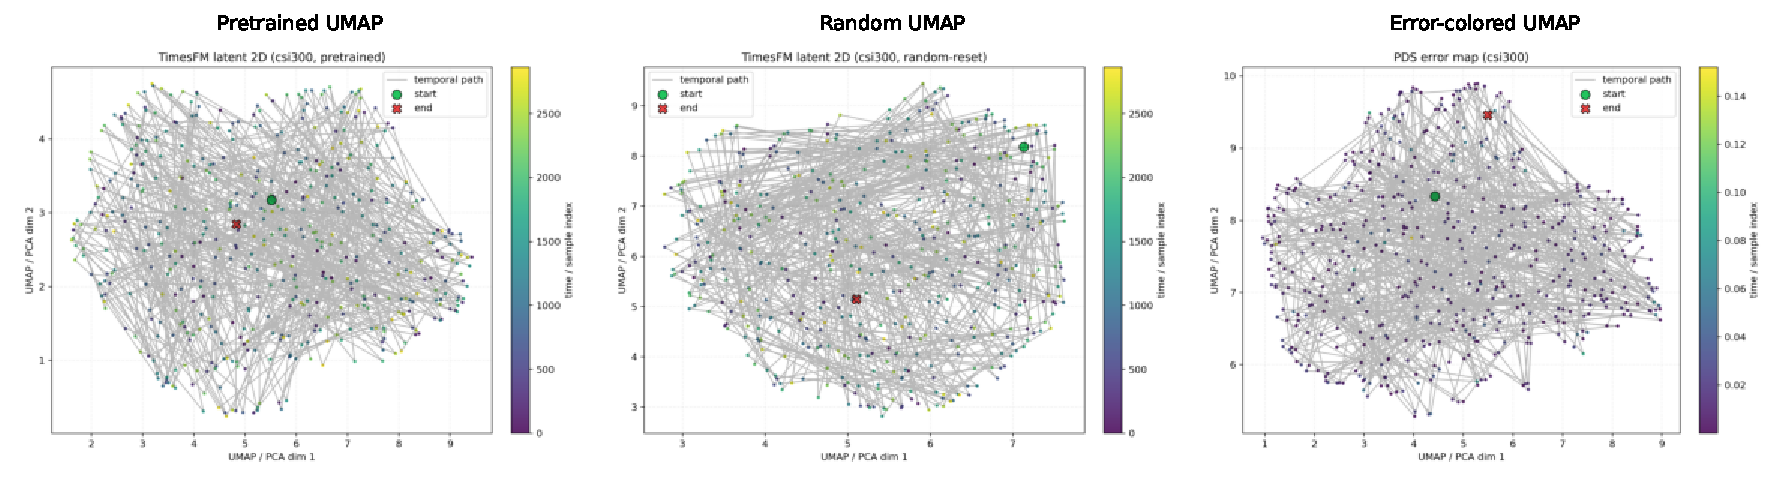
\includegraphics[width=\linewidth]{../outputs/figures/paper/fig_stock_ood}
\caption{Embedding geometry for OOD Chinese equity indices (CSI300 and CSI800).
\emph{Left two panels}: UMAP projections of pretrained TimesFM~2.0 embeddings
for CSI300 (top) and CSI800 (bottom), coloured by neighbourhood isolation
$\bar{d}_i$ (yellow~$=$~high isolation, purple~$=$~low).
\emph{Right two panels}: corresponding PDS scatter plots---neighbourhood
isolation $\bar{d}_i$ vs.\ absolute forecast error $|e_i|$---for pretrained
(blue) and random-weight (red) TimesFM.
In contrast to the Electricity manifold (Figure~\ref{fig:umap_electricity_app}),
where isolation varies substantially across the projection and tracks forecast
error, the equity embeddings produce \emph{uniform} high isolation across the
entire UMAP: every point is equally far from its neighbours.
This eliminates the variance in $\bar{d}_i$ required for a non-trivial
Spearman correlation, producing $\rho_s^{\mathrm{PDS}}{=}0.02$ (CSI300)
and $-0.09$ (CSI800), both indistinguishable from chance.}
\label{fig:stock_ood_app}
\end{figure}

The OOD equity figure provides the geometric explanation for the PDS collapse
quantified in Table~4 of the main paper.
The theoretical prediction (Theorem~5.1(ii), main paper; Corollary~\ref{cor:ood_pds}
of this appendix) is that when $d_{\mathcal{M}}(\mathcal{P}_{\mathrm{train}},
\mathcal{P}_{\mathrm{test}})$ is large, all OOD embeddings land in
low-density regions of $\trm$, making $\bar{d}_i$ uniformly large and its
Spearman correlation with $|e_i|$ near zero.

Figure~\ref{fig:stock_ood_app} confirms this picture directly.
The UMAP projections of CSI300 and CSI800 embeddings show a qualitatively
different structure from Electricity or Traffic: rather than a compact main
cluster with variable local density, the equity embeddings form a diffuse,
approximately uniform cloud.
The uniform colouration (all points yellow = high isolation) confirms that
the $k$-NN distances concentrate: Theorem~\ref{thm:knn_density}
($k$-NN Distance and Local Manifold Density) implies that if $\rho(z_i)$ is
uniformly low, then $\bar{d}_i^{(k)} \approx c_{\dint,k}\,\rho(z_i)^{-1/\dint}$
is uniformly large---and a near-constant variable has Spearman rank correlation
near zero with any other variable.

Crucially, this collapse is \emph{specific to the reliability signal}.
LTC$_{\mathrm{step}}$ remains above the random-weight baseline on both indices
(CSI300: $4.24$ vs.\ $3.80$; CSI800: $4.30$ vs.\ $3.82$), showing that the
encoder still organises temporal trajectories more richly than a random network.
CSS for seasonality and volatility are above chance ($p{<}0.05$) on both
indices, showing that these temporal primitives transfer out of distribution.
Only the local-density reliability signal fails---precisely because it depends
on a comparison of each test embedding to the training distribution's $\trm$,
a comparison that becomes uninformative when the test distribution is far from
training.

% ==============================================================
% Bibliography
% ==============================================================

\bibliographystyle{plainnat}
\begin{thebibliography}{20}

\bibitem[Ansuini et al.(2019)]{ansuini2019intrinsic}
Ansuini, A., Laio, A., Macke, J.~H., and Zoccolan, D.
\newblock Intrinsic dimension of data representations in deep neural networks.
\newblock In \emph{Advances in Neural Information Processing Systems}, 2019.

\bibitem[Birdal et al.(2021)]{birdal2021intrinsic}
Birdal, T., Lou, A., Guibas, L., and Simonovsky, M.
\newblock Intrinsic dimensionality explains the effectiveness of language model
  fine-tuning.
\newblock In \emph{Proceedings of the 59th Annual Meeting of the ACL}, 2021.

\bibitem[Bronstein et al.(2021)]{bronstein2021geometric}
Bronstein, M., Bruna, J., Cohen, T., and Veli{\v{c}}kovi{\'c}, P.
\newblock Geometric deep learning: Grids, groups, graphs, geodesics, and
  gauges.
\newblock \emph{arXiv preprint arXiv:2104.13478}, 2021.

\bibitem[Cover and Thomas(2006)]{cover2006information}
Cover, T.~M. and Thomas, J.~A.
\newblock \emph{Elements of Information Theory}.
\newblock John Wiley \& Sons, 2nd edition, 2006.

\bibitem[Facco et al.(2017)]{facco2017estimating}
Facco, E., d'Errico, M., Rodriguez, A., and Laio, A.
\newblock Estimating the intrinsic dimension of datasets by a minimal
  neighborhood information.
\newblock \emph{Scientific Reports}, 7(1), 2017.

\bibitem[Federer(1969)]{federer1969geometric}
Federer, H.
\newblock \emph{Geometric Measure Theory}.
\newblock Springer-Verlag, 1969.

\bibitem[Hardt et al.(2016)]{hardt2016train}
Hardt, M., Recht, B., and Singer, Y.
\newblock Train faster, generalize better: Stability of stochastic gradient
  descent.
\newblock In \emph{Proceedings of the 33rd International Conference on Machine
  Learning}, 2016.

\bibitem[Ledoux(2001)]{ledoux2001concentration}
Ledoux, M.
\newblock \emph{The Concentration of Measure Phenomenon}.
\newblock American Mathematical Society, 2001.

\bibitem[Penrose(2011)]{penrose2011random}
Penrose, M.
\newblock \emph{Random Geometric Graphs}.
\newblock Oxford University Press, 2011.

\bibitem[Raghu et al.(2017)]{raghu2017svcca}
Raghu, M., Gilmer, J., Yosinski, J., and Sohl-Dickstein, J.
\newblock {SVCCA}: Singular vector canonical correlation analysis for deep
  learning dynamics and interpretability.
\newblock In \emph{Advances in Neural Information Processing Systems}, 2017.

\bibitem[Reif et al.(2019)]{reif2019visualizing}
Reif, E., Yuan, A., Wattenberg, M., et al.
\newblock Visualizing and measuring the geometry of {BERT}.
\newblock In \emph{Advances in Neural Information Processing Systems}, 2019.

\bibitem[Shalev-Shwartz and Ben-David(2014)]{shalev2014understanding}
Shalev-Shwartz, S. and Ben-David, S.
\newblock \emph{Understanding Machine Learning: From Theory to Algorithms}.
\newblock Cambridge University Press, 2014.

\bibitem[Vershynin(2018)]{vershynin2018hdp}
Vershynin, R.
\newblock \emph{High-Dimensional Probability: An Introduction with Applications
  in Data Science}.
\newblock Cambridge University Press, 2018.

\end{thebibliography}

\end{document}
